\chapter{Descrição da solução}

Este projeto possui duas grandes partes, os Módulos Auxiliares (MA) e a central de controle. A figura \ref{dispositivos} mostra um diagrama geral de comunicação de um dispositivo acoplado a um Módulo Auxiliar (MA) com a central de controle.

\begin{figure}[H]
\caption{\label{dispositivos} Topologia da solução}
\includegraphics[scale=0.5]{img/arquitetura-basica-2.png}
\legend{Fonte: Autor do projeto}
\end{figure}

O principal diferencial deste projeto e a API de controle dos dispositivo, esta API segue o padrão RESt de implementação o que permite que qualquer cliente que tenha a capacidade de integrar-se a APIs deste tipo possam fazer uso dela.

\section{Módulos Auxiliares}
Estes módulos são acoplados a eletrodomésticos e são compostos por uma placa ESP8266 modelo ESP-01, todo processo de desenvolvimento do \textit{firmware} até a gravação deste \textit{firrmware} na placa ESP-01 é feito utilizando a IDE do Arduíno. Também são usados bibliotecas do framework Arduíno para comunicação através do protocolo MQTT com a central de controle.

\subsection{Esquema eletrônico do MA}
Foi desenvolvido um circuito para acoplar a placa ESP-01 a um relé, este é responsável por fazer o acionamento de cargas AC (Corrente Alternada, tradução do inglês). A figura \ref{sch-ma} mostra este circuíto de forma esquemática.

\begin{figure}[H]
\caption{\label{sch-ma} Esquemático eletrônico do MA}
\includegraphics[scale=0.25]{img/sch-ma.png}
\legend{Fonte: Autor do projeto}
\end{figure}

\subsection{Programação do \textit{firmware} do MA}
No processo de desenvolvimento do \textit{firmware} do MA foi utilizado a IDE Arduíno, a figura \ref{arduino-ide} mostra com um trecho do firmware de controle do MA.

\begin{figure}[H]
\caption{\label{arduino-ide} Arduíno IDE}
\includegraphics[scale=0.3]{img/ide-arduino.png}
\legend{Fonte: Autor do projeto}
\end{figure}

O processo de gravação do \textit{firmware} na placa ESP-01 utiliza um gravador que é acoplado a uma das portas USB do computador, a figura \ref{gravacao-firmware} mostra como é este gravador e a montagem do módulo para gravação de \textit{firmware}.

\begin{figure}[H]
\caption{\label{gravacao-firmware} Gravação do \textit{firmware} no MA}
\includegraphics[scale=0.11]{img/gravador-firmware.png}
\legend{Fonte: Autor do projeto}
\end{figure}

\section{Central de controle}
A central de controle é um micro computador com dimensões reduzidas, o modelo é uma RaspberryPI tipo B com 512MB de RAM e um cartão de memória do tipo SD card com 8GB de memória disponível. Neste computador estão instalados os seguintes programas:

\begin{itemize}
    \item[a)] Sistema operacional Debian na versão 8;
    \item[b)] Broker MQTT Mosquitto versão 1.4.14;
    \item[c)] NodeJS versão 8.2.1;
    \item[d)] Sqlite3 versão 3.8.7.
\end{itemize}

Na figura \ref{raspberry-case} é possível ver o computador montado em uma caixa de acrílico.

\begin{figure}[H]
\caption{\label{raspberry-case} Central de controle}
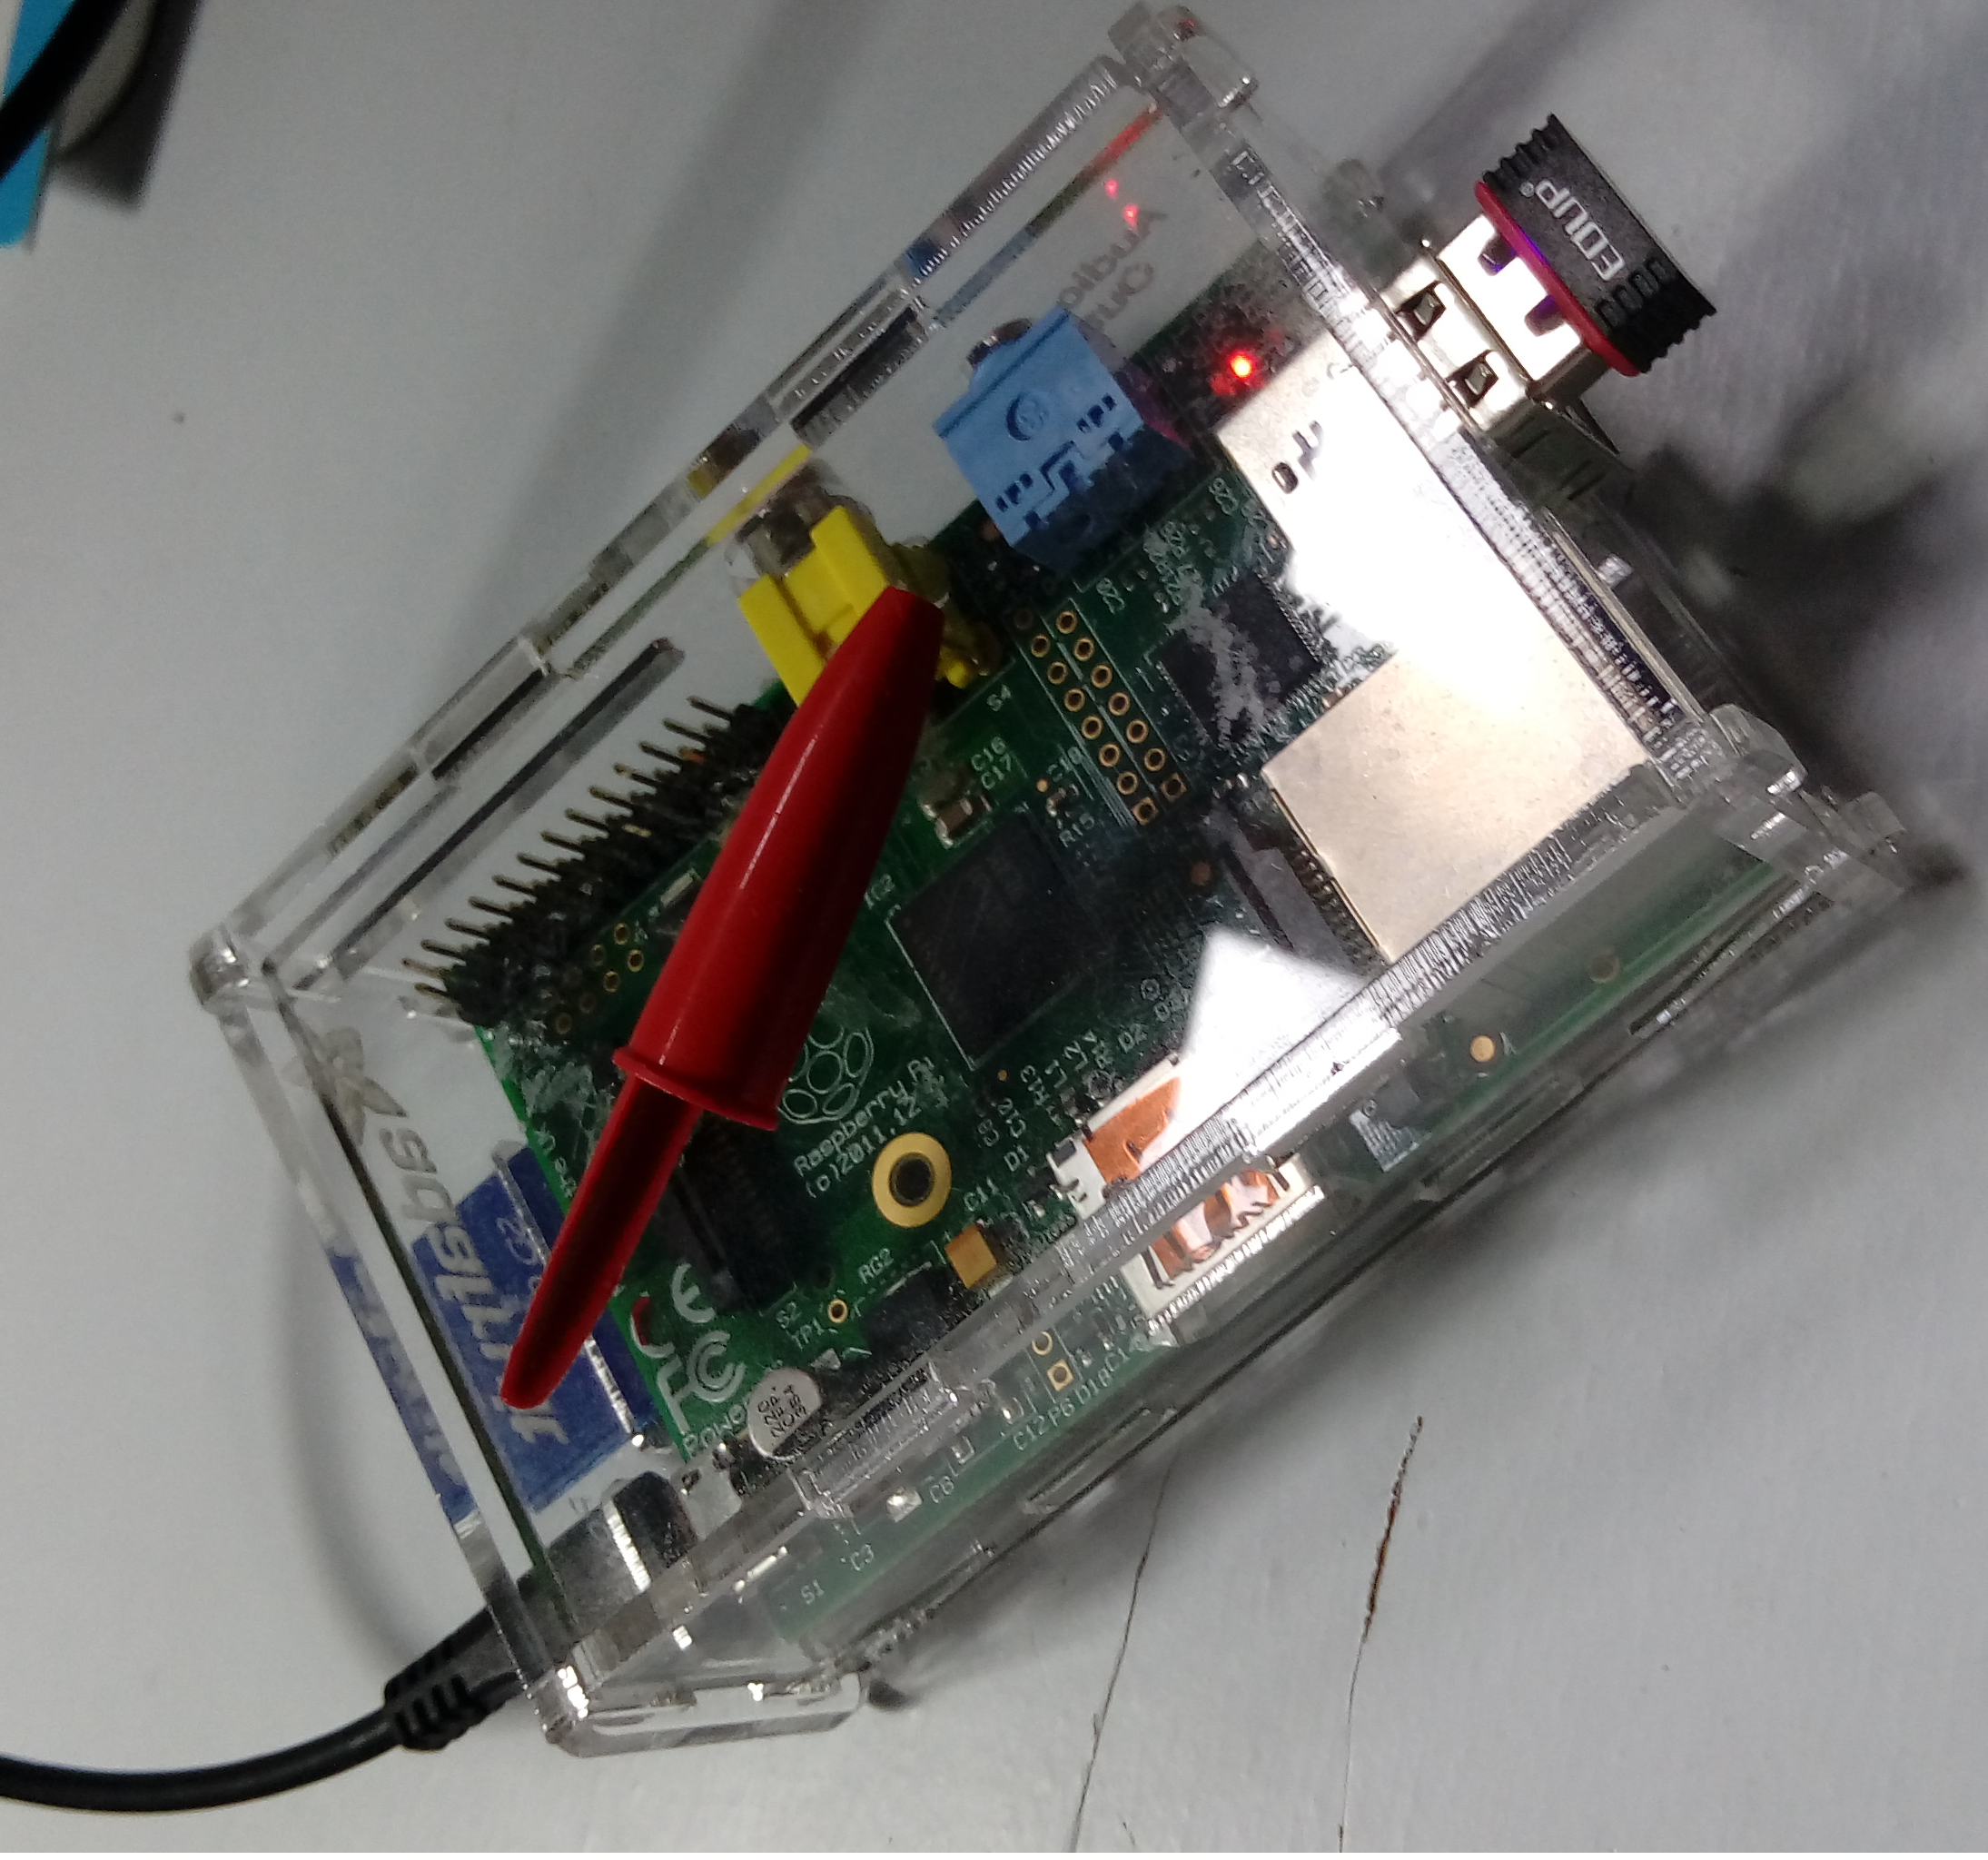
\includegraphics[scale=0.15]{img/rpi.png}
\legend{Fonte: Autor do projeto}
\end{figure}

Na figura \ref{ysto-central} mostra a coleção de serviços e aplicativos que estão hospedados na central de controle.

\begin{figure}[H]
\caption{\label{ysto-central} Esquemático de serviços da central de controle}
\includegraphics[scale=0.5]{img/ysto-diagrama-central.png}
\legend{Fonte: Autor do projeto}
\end{figure}

A troca de mensagens será feita utilizando o protocolo chamado Telemetry Transport Message Queue (MQTT), este protocolo além de possuir um baixo consumo de banda (as mensagens são relativamente pequenas em comparação com outros protocolos que trafegam no mesmo meio, http por exemplo) ainda fornece ferramentas necessárias para:

\begin{itemize}
    \item[a)] Fazer o controle de quem pode trocar mensagens na nossa rede de dispositivos;
    \item[b)] Garantir a entrega das mensagens;
    \item[c)] Integração com aplicativos de mercado em diversas plataformas mobile ou \textit{Desktop}.
\end{itemize}

Este Dashboard será um Appweb do tipo \textit{Mobile First} ou seja, seus layouts serão adaptados para as telas de telefones, tablets e computadores.

\section{Funcionamento do protocolo MQTT}
Este projeto baseia-se fortemente no funcionamento do protocolo MQTT (IBM, 2017), é importante entender como este funciona pois tem reflexo direto em como este projeto opera. Este protocolo de comunicação permite estabelecer uma maneira simples de comunicação entre múltiplos dispositivos, podendo:

\begin{itemize}
    \item[a)] Enviar um comando para uma saída;
    \item[b)] Ler uma entrada e publicar os dados lidos.
\end{itemize}

A figura \ref{mqtt-1} exemplifica o funcionamento do envio de um comando para uma saída do sistema.

\begin{figure}[H]
\caption{\label{mqtt-1} Mensagem sendo enviada via MQTT}
\includegraphics[scale=0.5]{img/mqtt-1.png}
\legend{Fonte: Random Nerd Tutorials}
\end{figure}

Já figura \ref{mqtt-2} demonstra o recebimento de dados de um sensor de temperatura.

\begin{figure}[H]
\caption{\label{mqtt-2} Mensagem sendo recebida via MQTT}
\includegraphics[scale=0.5]{img/mqtt-2.png}
\legend{Fonte: Random Nerd Tutorials}
\end{figure}

Existem alguns conceitos básicos que envolvem o uso deste protocolo, são eles:

\begin{itemize}
    \item[a)] Publish/Subscribe : Um dispositivo pode publicar mensagens para outros dispositivos, ou um dispositivo pode ser inscrever em um tópico qualquer e passa a receber as mensagens deste tópico;
    \item[b)] Messages: São as informações trocadas entre os dispositivos, podem ser comandos ou apenas informações;
    \item[c)] Topics: É a maneira como um dispositivo demonstra interesse em determinadas mensagens, pode também ser definido como o lugar onde um dispositivo deseja publicar suas mensagens;
    \item[d)] Broker: É o responsável por receber todas as mensagens, fazer o filtro e publicar nos respectivos tópicos.
\end{itemize}

A figura \ref{mqtt-3} demonstra de forma esquemática as diversas ações que ocorrem durante uma troca de mensagens entre dispositivos.

\begin{figure}[H]
\caption{\label{mqtt-3} Modelo publish/subscribe}
\includegraphics[scale=0.25]{img/mqtt-3.png}
\legend{Fonte: Random Nerd Tutorials}
\end{figure}

A figura \ref{mqtt-4} mostra como uma estrutura de tópicos pode ser montada para fazer o acionamento de um dispositivo, no caso uma lâmpada.

\begin{figure}[H]
\caption{\label{mqtt-4} Um exemplo de estrutura de tópicos}
\includegraphics[scale=0.3]{img/mqtt-5.png}
\legend{Fonte: Random Nerd Tutorials}
\end{figure}

A figura \ref{mqtt-5} mostra o papel do Broker dentro deste cenário.

\begin{figure}[H]
\caption{\label{mqtt-5} O papel do broker}
\includegraphics[scale=0.25]{img/mqtt-4.png}
\legend{Fonte: Random Nerd Tutorials}
\end{figure}

\subsection{Tópico para controle de um MA}
De acordo com o descrito na seção de descrição da solução, este projeto está baseado no conceito \textit{Publish/Subscribe} onde uma estrutura de tópicos é necessária para a execução de ações e coleta de dados, a figura \ref{mqtt-6} mostra como é nossa estrutura de tópicos.

\begin{figure}[H]
\caption{\label{mqtt-6} Estrutura de tópicos adotada neste projeto}
\includegraphics[scale=0.25]{img/topicos.png}
\legend{Fonte: Random Nerd Tutorials}
\end{figure}

\section{Ponto de entrada no sistema}
Para os usuários ou administradores do sistema, tudo será controlado por acesso a URL da rede local, no endereço http://ysto.local. Basta então, através do seu apontar para este endereço estando conectado a rede local do ysto.






